\documentclass[twoside]{book}

% Packages required by doxygen
\usepackage{fixltx2e}
\usepackage{calc}
\usepackage{doxygen}
\usepackage[export]{adjustbox} % also loads graphicx
\usepackage{graphicx}
\usepackage[utf8]{inputenc}
\usepackage{makeidx}
\usepackage{multicol}
\usepackage{multirow}
\PassOptionsToPackage{warn}{textcomp}
\usepackage{textcomp}
\usepackage[nointegrals]{wasysym}
\usepackage[table]{xcolor}

% Font selection
\usepackage[T1]{fontenc}
\usepackage[scaled=.90]{helvet}
\usepackage{courier}
\usepackage{amssymb}
\usepackage{sectsty}
\renewcommand{\familydefault}{\sfdefault}
\allsectionsfont{%
  \fontseries{bc}\selectfont%
  \color{darkgray}%
}
\renewcommand{\DoxyLabelFont}{%
  \fontseries{bc}\selectfont%
  \color{darkgray}%
}
\newcommand{\+}{\discretionary{\mbox{\scriptsize$\hookleftarrow$}}{}{}}

% Page & text layout
\usepackage{geometry}
\geometry{%
  a4paper,%
  top=2.5cm,%
  bottom=2.5cm,%
  left=2.5cm,%
  right=2.5cm%
}
\tolerance=750
\hfuzz=15pt
\hbadness=750
\setlength{\emergencystretch}{15pt}
\setlength{\parindent}{0cm}
\setlength{\parskip}{0.2cm}
\makeatletter
\renewcommand{\paragraph}{%
  \@startsection{paragraph}{4}{0ex}{-1.0ex}{1.0ex}{%
    \normalfont\normalsize\bfseries\SS@parafont%
  }%
}
\renewcommand{\subparagraph}{%
  \@startsection{subparagraph}{5}{0ex}{-1.0ex}{1.0ex}{%
    \normalfont\normalsize\bfseries\SS@subparafont%
  }%
}
\makeatother

% Headers & footers
\usepackage{fancyhdr}
\pagestyle{fancyplain}
\fancyhead[LE]{\fancyplain{}{\bfseries\thepage}}
\fancyhead[CE]{\fancyplain{}{}}
\fancyhead[RE]{\fancyplain{}{\bfseries\leftmark}}
\fancyhead[LO]{\fancyplain{}{\bfseries\rightmark}}
\fancyhead[CO]{\fancyplain{}{}}
\fancyhead[RO]{\fancyplain{}{\bfseries\thepage}}
\fancyfoot[LE]{\fancyplain{}{}}
\fancyfoot[CE]{\fancyplain{}{}}
\fancyfoot[RE]{\fancyplain{}{\bfseries\scriptsize Generated on Sun Jan 25 2015 23\+:15\+:06 for W\+Y\+D\+A\+T\+K\+I by Doxygen }}
\fancyfoot[LO]{\fancyplain{}{\bfseries\scriptsize Generated on Sun Jan 25 2015 23\+:15\+:06 for W\+Y\+D\+A\+T\+K\+I by Doxygen }}
\fancyfoot[CO]{\fancyplain{}{}}
\fancyfoot[RO]{\fancyplain{}{}}
\renewcommand{\footrulewidth}{0.4pt}
\renewcommand{\chaptermark}[1]{%
  \markboth{#1}{}%
}
\renewcommand{\sectionmark}[1]{%
  \markright{\thesection\ #1}%
}

% Indices & bibliography
\usepackage{natbib}
\usepackage[titles]{tocloft}
\setcounter{tocdepth}{3}
\setcounter{secnumdepth}{5}
\makeindex

% Hyperlinks (required, but should be loaded last)
\usepackage{ifpdf}
\ifpdf
  \usepackage[pdftex,pagebackref=true]{hyperref}
\else
  \usepackage[ps2pdf,pagebackref=true]{hyperref}
\fi
\hypersetup{%
  colorlinks=true,%
  linkcolor=blue,%
  citecolor=blue,%
  unicode%
}

% Custom commands
\newcommand{\clearemptydoublepage}{%
  \newpage{\pagestyle{empty}\cleardoublepage}%
}


%===== C O N T E N T S =====

\begin{document}

% Titlepage & ToC
\hypersetup{pageanchor=false,
             bookmarks=true,
             bookmarksnumbered=true,
             pdfencoding=unicode
            }
\pagenumbering{roman}
\begin{titlepage}
\vspace*{7cm}
\begin{center}%
{\Large W\+Y\+D\+A\+T\+K\+I \\[1ex]\large 1.\+0 }\\
\vspace*{1cm}
{\large Generated by Doxygen 1.8.9.1}\\
\vspace*{0.5cm}
{\small Sun Jan 25 2015 23:15:06}\\
\end{center}
\end{titlepage}
\clearemptydoublepage
\tableofcontents
\clearemptydoublepage
\pagenumbering{arabic}
\hypersetup{pageanchor=true}

%--- Begin generated contents ---
\chapter{Hierarchical Index}
\section{Class Hierarchy}
This inheritance list is sorted roughly, but not completely, alphabetically\+:\begin{DoxyCompactList}
\item \contentsline{section}{Lista\+Kategorii}{\pageref{class_lista_kategorii}}{}
\item \contentsline{section}{Lista\+Wydatkow}{\pageref{class_lista_wydatkow}}{}
\item \contentsline{section}{Menager\+Wydatkow}{\pageref{class_menager_wydatkow}}{}
\item Q\+Dialog\begin{DoxyCompactList}
\item \contentsline{section}{Dialog\+Dodaj}{\pageref{class_dialog_dodaj}}{}
\end{DoxyCompactList}
\item Q\+Main\+Window\begin{DoxyCompactList}
\item \contentsline{section}{Main\+Window}{\pageref{class_main_window}}{}
\end{DoxyCompactList}
\item \contentsline{section}{Wpis\+Zestawienia}{\pageref{class_wpis_zestawienia}}{}
\item \contentsline{section}{Wydatek}{\pageref{class_wydatek}}{}
\item \contentsline{section}{Zestawienie}{\pageref{class_zestawienie}}{}
\end{DoxyCompactList}

\chapter{Class Index}
\section{Class List}
Here are the classes, structs, unions and interfaces with brief descriptions\+:\begin{DoxyCompactList}
\item\contentsline{section}{\hyperlink{class_dialog_dodaj}{Dialog\+Dodaj} \\*Klasa \hyperlink{class_dialog_dodaj}{Dialog\+Dodaj}. Klasa wyswietla okienko do dodawania wpisu }{\pageref{class_dialog_dodaj}}{}
\item\contentsline{section}{\hyperlink{class_lista_kategorii}{Lista\+Kategorii} \\*Klasa \hyperlink{class_lista_kategorii}{Lista\+Kategorii}. Klasa ktora uniemozliwia duplikacje kategorii }{\pageref{class_lista_kategorii}}{}
\item\contentsline{section}{\hyperlink{class_lista_wydatkow}{Lista\+Wydatkow} \\*Klasa \hyperlink{class_lista_wydatkow}{Lista\+Wydatkow}. Klasa przechowujaca liste wydatkow }{\pageref{class_lista_wydatkow}}{}
\item\contentsline{section}{\hyperlink{class_main_window}{Main\+Window} \\*Klasa \hyperlink{class_main_window}{Main\+Window}. Klasa wyswietlajaca okno glowne }{\pageref{class_main_window}}{}
\item\contentsline{section}{\hyperlink{class_menager_wydatkow}{Menager\+Wydatkow} \\*Klasa \hyperlink{class_menager_wydatkow}{Menager\+Wydatkow}. Klasa zawierajaca wszystkie listy i laczaca sie z baza }{\pageref{class_menager_wydatkow}}{}
\item\contentsline{section}{\hyperlink{class_wpis_zestawienia}{Wpis\+Zestawienia} \\*Klasa \hyperlink{class_wpis_zestawienia}{Wpis\+Zestawienia}. Klasa reprezentujaca pojedynczy wpis z zestawienia }{\pageref{class_wpis_zestawienia}}{}
\item\contentsline{section}{\hyperlink{class_wydatek}{Wydatek} \\*Klasa \hyperlink{class_wydatek}{Wydatek}. Klasa reprezentujaca pojedynczy wpis }{\pageref{class_wydatek}}{}
\item\contentsline{section}{\hyperlink{class_zestawienie}{Zestawienie} }{\pageref{class_zestawienie}}{}
\end{DoxyCompactList}

\chapter{Class Documentation}
\hypertarget{class_dialog_dodaj}{}\section{Dialog\+Dodaj Class Reference}
\label{class_dialog_dodaj}\index{Dialog\+Dodaj@{Dialog\+Dodaj}}


Klasa \hyperlink{class_dialog_dodaj}{Dialog\+Dodaj}. Klasa wyswietla okienko do dodawania wpisu.  




{\ttfamily \#include $<$dialogdodaj.\+h$>$}



Inheritance diagram for Dialog\+Dodaj\+:\nopagebreak
\begin{figure}[H]
\begin{center}
\leavevmode
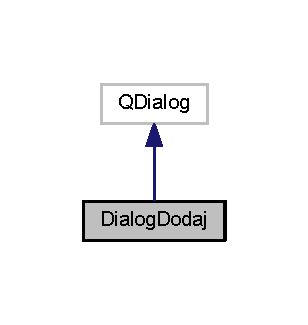
\includegraphics[width=148pt]{class_dialog_dodaj__inherit__graph}
\end{center}
\end{figure}


Collaboration diagram for Dialog\+Dodaj\+:\nopagebreak
\begin{figure}[H]
\begin{center}
\leavevmode
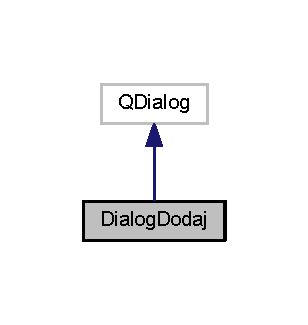
\includegraphics[width=148pt]{class_dialog_dodaj__coll__graph}
\end{center}
\end{figure}
\subsection*{Public Member Functions}
\begin{DoxyCompactItemize}
\item 
\hyperlink{class_dialog_dodaj_ad0b34b49b64f5a80112be0ad90af8f79}{Dialog\+Dodaj} (Q\+Widget $\ast$parent=0)
\begin{DoxyCompactList}\small\item\em Konstruktor \hyperlink{class_dialog_dodaj}{Dialog\+Dodaj}. Zamyka okno dodawania jesli wylaczamy program. \end{DoxyCompactList}\item 
void \hyperlink{class_dialog_dodaj_a8c6c561a5a1427422ed8e6c3be794aaf}{set\+Lista\+Kategorii} (Q\+String\+List lista\+Kat)
\begin{DoxyCompactList}\small\item\em Funkcja set\+Lista\+Kategorii. Przyjmuje argument Lista\+Kat. Dodaje kategorie do listy. \end{DoxyCompactList}\item 
Q\+String \hyperlink{class_dialog_dodaj_a730c587aec50f9a1fa092597ade172df}{get\+Kategoria} ()
\begin{DoxyCompactList}\small\item\em Funkcja get\+Kategoria umozliwia wpisywanie kategorii w okienku. \end{DoxyCompactList}\item 
Q\+Date \hyperlink{class_dialog_dodaj_ad7e955de6adf2bd0dfe001c6973010d3}{get\+Data} ()
\begin{DoxyCompactList}\small\item\em Funkcja get\+Data umozliwia wpisywanie daty w okienku. \end{DoxyCompactList}\item 
double \hyperlink{class_dialog_dodaj_a105359d1ef27ae66ec5e0ed6d7272e37}{get\+Kwota} ()
\begin{DoxyCompactList}\small\item\em Funkcja get\+Kwota umozliwia wpisywanie kwoty w okienku. \end{DoxyCompactList}\item 
Q\+String \hyperlink{class_dialog_dodaj_ab3738341a33051b2d817400c2d7239a3}{get\+Opis} ()
\begin{DoxyCompactList}\small\item\em Funkcja get\+Opis umozliwia wpisywanie opis w okienku. \end{DoxyCompactList}\item 
void \hyperlink{class_dialog_dodaj_a9c50df1e504afc4770393a8d408513da}{set\+Kategoria} (Q\+String kategoria)
\begin{DoxyCompactList}\small\item\em Funkcja set\+Kategoria. Przyjmuje argument kategoria. przechowuje obecna kategorie wpisana w polu tekstowym. \end{DoxyCompactList}\item 
void \hyperlink{class_dialog_dodaj_aa841614497235c9464d84e031748a6fd}{set\+Data} (Q\+Date data)
\begin{DoxyCompactList}\small\item\em Funkcja set\+Data przechowuje obecna date wpisana w polu tekstowym. \end{DoxyCompactList}\item 
void \hyperlink{class_dialog_dodaj_a8b16a52786c9b6ac4ab2728256b3b783}{set\+Kwota} (double kwota)
\begin{DoxyCompactList}\small\item\em Funkcja set\+Kwota przechowuje obecna kwote wpisana w polu tekstowym. \end{DoxyCompactList}\item 
void \hyperlink{class_dialog_dodaj_a63119933c54c3b316b242697c2c2cf9c}{set\+Opis} (Q\+String opis)
\begin{DoxyCompactList}\small\item\em Funkcja set\+Opis. Przyjmuje argument opis. przechowuje obecny opis wpisany w polu tekstowym. \end{DoxyCompactList}\end{DoxyCompactItemize}


\subsection{Detailed Description}
Klasa \hyperlink{class_dialog_dodaj}{Dialog\+Dodaj}. Klasa wyswietla okienko do dodawania wpisu. 

\subsection{Constructor \& Destructor Documentation}
\hypertarget{class_dialog_dodaj_ad0b34b49b64f5a80112be0ad90af8f79}{}\index{Dialog\+Dodaj@{Dialog\+Dodaj}!Dialog\+Dodaj@{Dialog\+Dodaj}}
\index{Dialog\+Dodaj@{Dialog\+Dodaj}!Dialog\+Dodaj@{Dialog\+Dodaj}}
\subsubsection[{Dialog\+Dodaj}]{\setlength{\rightskip}{0pt plus 5cm}Dialog\+Dodaj\+::\+Dialog\+Dodaj (
\begin{DoxyParamCaption}
\item[{Q\+Widget $\ast$}]{parent = {\ttfamily 0}}
\end{DoxyParamCaption}
)\hspace{0.3cm}{\ttfamily [explicit]}}\label{class_dialog_dodaj_ad0b34b49b64f5a80112be0ad90af8f79}


Konstruktor \hyperlink{class_dialog_dodaj}{Dialog\+Dodaj}. Zamyka okno dodawania jesli wylaczamy program. 


\begin{DoxyParams}{Parameters}
{\em parent} & \\
\hline
\end{DoxyParams}


\subsection{Member Function Documentation}
\hypertarget{class_dialog_dodaj_ad7e955de6adf2bd0dfe001c6973010d3}{}\index{Dialog\+Dodaj@{Dialog\+Dodaj}!get\+Data@{get\+Data}}
\index{get\+Data@{get\+Data}!Dialog\+Dodaj@{Dialog\+Dodaj}}
\subsubsection[{get\+Data}]{\setlength{\rightskip}{0pt plus 5cm}Q\+Date Dialog\+Dodaj\+::get\+Data (
\begin{DoxyParamCaption}
{}
\end{DoxyParamCaption}
)}\label{class_dialog_dodaj_ad7e955de6adf2bd0dfe001c6973010d3}


Funkcja get\+Data umozliwia wpisywanie daty w okienku. 

\begin{DoxyReturn}{Returns}
Zwraca zmienna typu Q\+Date. 
\end{DoxyReturn}
\hypertarget{class_dialog_dodaj_a730c587aec50f9a1fa092597ade172df}{}\index{Dialog\+Dodaj@{Dialog\+Dodaj}!get\+Kategoria@{get\+Kategoria}}
\index{get\+Kategoria@{get\+Kategoria}!Dialog\+Dodaj@{Dialog\+Dodaj}}
\subsubsection[{get\+Kategoria}]{\setlength{\rightskip}{0pt plus 5cm}Q\+String Dialog\+Dodaj\+::get\+Kategoria (
\begin{DoxyParamCaption}
{}
\end{DoxyParamCaption}
)}\label{class_dialog_dodaj_a730c587aec50f9a1fa092597ade172df}


Funkcja get\+Kategoria umozliwia wpisywanie kategorii w okienku. 

\begin{DoxyReturn}{Returns}
Zwraca zmienna typu Q\+String. 
\end{DoxyReturn}
\hypertarget{class_dialog_dodaj_a105359d1ef27ae66ec5e0ed6d7272e37}{}\index{Dialog\+Dodaj@{Dialog\+Dodaj}!get\+Kwota@{get\+Kwota}}
\index{get\+Kwota@{get\+Kwota}!Dialog\+Dodaj@{Dialog\+Dodaj}}
\subsubsection[{get\+Kwota}]{\setlength{\rightskip}{0pt plus 5cm}double Dialog\+Dodaj\+::get\+Kwota (
\begin{DoxyParamCaption}
{}
\end{DoxyParamCaption}
)}\label{class_dialog_dodaj_a105359d1ef27ae66ec5e0ed6d7272e37}


Funkcja get\+Kwota umozliwia wpisywanie kwoty w okienku. 

\begin{DoxyReturn}{Returns}
Zwraca zmienna typu double. 
\end{DoxyReturn}
\hypertarget{class_dialog_dodaj_ab3738341a33051b2d817400c2d7239a3}{}\index{Dialog\+Dodaj@{Dialog\+Dodaj}!get\+Opis@{get\+Opis}}
\index{get\+Opis@{get\+Opis}!Dialog\+Dodaj@{Dialog\+Dodaj}}
\subsubsection[{get\+Opis}]{\setlength{\rightskip}{0pt plus 5cm}Q\+String Dialog\+Dodaj\+::get\+Opis (
\begin{DoxyParamCaption}
{}
\end{DoxyParamCaption}
)}\label{class_dialog_dodaj_ab3738341a33051b2d817400c2d7239a3}


Funkcja get\+Opis umozliwia wpisywanie opis w okienku. 

\begin{DoxyReturn}{Returns}
Zwraca zmienna typu Q\+String. 
\end{DoxyReturn}
\hypertarget{class_dialog_dodaj_aa841614497235c9464d84e031748a6fd}{}\index{Dialog\+Dodaj@{Dialog\+Dodaj}!set\+Data@{set\+Data}}
\index{set\+Data@{set\+Data}!Dialog\+Dodaj@{Dialog\+Dodaj}}
\subsubsection[{set\+Data}]{\setlength{\rightskip}{0pt plus 5cm}void Dialog\+Dodaj\+::set\+Data (
\begin{DoxyParamCaption}
\item[{Q\+Date}]{data}
\end{DoxyParamCaption}
)}\label{class_dialog_dodaj_aa841614497235c9464d84e031748a6fd}


Funkcja set\+Data przechowuje obecna date wpisana w polu tekstowym. 


\begin{DoxyParams}{Parameters}
{\em data} & jest argumentem typu Q\+Date. \\
\hline
\end{DoxyParams}
\hypertarget{class_dialog_dodaj_a9c50df1e504afc4770393a8d408513da}{}\index{Dialog\+Dodaj@{Dialog\+Dodaj}!set\+Kategoria@{set\+Kategoria}}
\index{set\+Kategoria@{set\+Kategoria}!Dialog\+Dodaj@{Dialog\+Dodaj}}
\subsubsection[{set\+Kategoria}]{\setlength{\rightskip}{0pt plus 5cm}void Dialog\+Dodaj\+::set\+Kategoria (
\begin{DoxyParamCaption}
\item[{Q\+String}]{kategoria}
\end{DoxyParamCaption}
)}\label{class_dialog_dodaj_a9c50df1e504afc4770393a8d408513da}


Funkcja set\+Kategoria. Przyjmuje argument kategoria. przechowuje obecna kategorie wpisana w polu tekstowym. 


\begin{DoxyParams}{Parameters}
{\em kategoria} & jest argumentem typu Q\+String. \\
\hline
\end{DoxyParams}
\hypertarget{class_dialog_dodaj_a8b16a52786c9b6ac4ab2728256b3b783}{}\index{Dialog\+Dodaj@{Dialog\+Dodaj}!set\+Kwota@{set\+Kwota}}
\index{set\+Kwota@{set\+Kwota}!Dialog\+Dodaj@{Dialog\+Dodaj}}
\subsubsection[{set\+Kwota}]{\setlength{\rightskip}{0pt plus 5cm}void Dialog\+Dodaj\+::set\+Kwota (
\begin{DoxyParamCaption}
\item[{double}]{kwota}
\end{DoxyParamCaption}
)}\label{class_dialog_dodaj_a8b16a52786c9b6ac4ab2728256b3b783}


Funkcja set\+Kwota przechowuje obecna kwote wpisana w polu tekstowym. 


\begin{DoxyParams}{Parameters}
{\em kwota} & jest argumentem typu double. \\
\hline
\end{DoxyParams}
\hypertarget{class_dialog_dodaj_a8c6c561a5a1427422ed8e6c3be794aaf}{}\index{Dialog\+Dodaj@{Dialog\+Dodaj}!set\+Lista\+Kategorii@{set\+Lista\+Kategorii}}
\index{set\+Lista\+Kategorii@{set\+Lista\+Kategorii}!Dialog\+Dodaj@{Dialog\+Dodaj}}
\subsubsection[{set\+Lista\+Kategorii}]{\setlength{\rightskip}{0pt plus 5cm}void Dialog\+Dodaj\+::set\+Lista\+Kategorii (
\begin{DoxyParamCaption}
\item[{Q\+String\+List}]{lista\+Kat}
\end{DoxyParamCaption}
)}\label{class_dialog_dodaj_a8c6c561a5a1427422ed8e6c3be794aaf}


Funkcja set\+Lista\+Kategorii. Przyjmuje argument Lista\+Kat. Dodaje kategorie do listy. 


\begin{DoxyParams}{Parameters}
{\em lista\+Kat} & jest argumentem typu Q\+String\+List. \\
\hline
\end{DoxyParams}
\hypertarget{class_dialog_dodaj_a63119933c54c3b316b242697c2c2cf9c}{}\index{Dialog\+Dodaj@{Dialog\+Dodaj}!set\+Opis@{set\+Opis}}
\index{set\+Opis@{set\+Opis}!Dialog\+Dodaj@{Dialog\+Dodaj}}
\subsubsection[{set\+Opis}]{\setlength{\rightskip}{0pt plus 5cm}void Dialog\+Dodaj\+::set\+Opis (
\begin{DoxyParamCaption}
\item[{Q\+String}]{opis}
\end{DoxyParamCaption}
)}\label{class_dialog_dodaj_a63119933c54c3b316b242697c2c2cf9c}


Funkcja set\+Opis. Przyjmuje argument opis. przechowuje obecny opis wpisany w polu tekstowym. 


\begin{DoxyParams}{Parameters}
{\em opis} & jest argumentem typu Q\+String. \\
\hline
\end{DoxyParams}


The documentation for this class was generated from the following files\+:\begin{DoxyCompactItemize}
\item 
dialogdodaj.\+h\item 
dialogdodaj.\+cpp\end{DoxyCompactItemize}

\hypertarget{class_lista_kategorii}{}\section{Lista\+Kategorii Class Reference}
\label{class_lista_kategorii}\index{Lista\+Kategorii@{Lista\+Kategorii}}


Klasa \hyperlink{class_lista_kategorii}{Lista\+Kategorii}. Klasa ktora uniemozliwia duplikacje kategorii.  




{\ttfamily \#include $<$listakategorii.\+h$>$}

\subsection*{Public Member Functions}
\begin{DoxyCompactItemize}
\item 
\hypertarget{class_lista_kategorii_acef65dde16520b6ff29ccba87c2e1165}{}\hyperlink{class_lista_kategorii_acef65dde16520b6ff29ccba87c2e1165}{Lista\+Kategorii} ()\label{class_lista_kategorii_acef65dde16520b6ff29ccba87c2e1165}

\begin{DoxyCompactList}\small\item\em Konstruktor \hyperlink{class_lista_kategorii}{Lista\+Kategorii}. \end{DoxyCompactList}\item 
bool \hyperlink{class_lista_kategorii_a76d076d87408f34c36fd4e2c56d010e1}{dodaj} (Q\+String str)
\begin{DoxyCompactList}\small\item\em Funkcja dodaj. Przyjmuje argument str. Sprawdza czy nowa kategoria zostala dodana. \end{DoxyCompactList}\item 
bool \hyperlink{class_lista_kategorii_a1ae1a558622fb75c33f22e1e897c0ac4}{usun} (Q\+String str)
\begin{DoxyCompactList}\small\item\em Funkcja usun. Przyjmuje argument str. Sprawdza czy kategoria zostala usunieta. \end{DoxyCompactList}\item 
Q\+String\+List \hyperlink{class_lista_kategorii_a82324bbd533f8e6395afc0b3e4babef8}{get\+List} ()
\begin{DoxyCompactList}\small\item\em Funkcja get\+List. Pobiera liste kategorii. \end{DoxyCompactList}\end{DoxyCompactItemize}


\subsection{Detailed Description}
Klasa \hyperlink{class_lista_kategorii}{Lista\+Kategorii}. Klasa ktora uniemozliwia duplikacje kategorii. 

\subsection{Member Function Documentation}
\hypertarget{class_lista_kategorii_a76d076d87408f34c36fd4e2c56d010e1}{}\index{Lista\+Kategorii@{Lista\+Kategorii}!dodaj@{dodaj}}
\index{dodaj@{dodaj}!Lista\+Kategorii@{Lista\+Kategorii}}
\subsubsection[{dodaj}]{\setlength{\rightskip}{0pt plus 5cm}bool Lista\+Kategorii\+::dodaj (
\begin{DoxyParamCaption}
\item[{Q\+String}]{str}
\end{DoxyParamCaption}
)}\label{class_lista_kategorii_a76d076d87408f34c36fd4e2c56d010e1}


Funkcja dodaj. Przyjmuje argument str. Sprawdza czy nowa kategoria zostala dodana. 


\begin{DoxyParams}{Parameters}
{\em Argument} & str jest typu Q\+String. \\
\hline
\end{DoxyParams}
\begin{DoxyReturn}{Returns}
Zwraca zmienna typu bool. 
\end{DoxyReturn}
\hypertarget{class_lista_kategorii_a82324bbd533f8e6395afc0b3e4babef8}{}\index{Lista\+Kategorii@{Lista\+Kategorii}!get\+List@{get\+List}}
\index{get\+List@{get\+List}!Lista\+Kategorii@{Lista\+Kategorii}}
\subsubsection[{get\+List}]{\setlength{\rightskip}{0pt plus 5cm}Q\+String\+List Lista\+Kategorii\+::get\+List (
\begin{DoxyParamCaption}
{}
\end{DoxyParamCaption}
)}\label{class_lista_kategorii_a82324bbd533f8e6395afc0b3e4babef8}


Funkcja get\+List. Pobiera liste kategorii. 

\begin{DoxyReturn}{Returns}
Zwraca obiekt typu Q\+String\+List. 
\end{DoxyReturn}
\hypertarget{class_lista_kategorii_a1ae1a558622fb75c33f22e1e897c0ac4}{}\index{Lista\+Kategorii@{Lista\+Kategorii}!usun@{usun}}
\index{usun@{usun}!Lista\+Kategorii@{Lista\+Kategorii}}
\subsubsection[{usun}]{\setlength{\rightskip}{0pt plus 5cm}bool Lista\+Kategorii\+::usun (
\begin{DoxyParamCaption}
\item[{Q\+String}]{str}
\end{DoxyParamCaption}
)}\label{class_lista_kategorii_a1ae1a558622fb75c33f22e1e897c0ac4}


Funkcja usun. Przyjmuje argument str. Sprawdza czy kategoria zostala usunieta. 


\begin{DoxyParams}{Parameters}
{\em Argument} & str jest typu Q\+String. \\
\hline
\end{DoxyParams}
\begin{DoxyReturn}{Returns}
Zwraca zmienna typu bool. 
\end{DoxyReturn}


The documentation for this class was generated from the following files\+:\begin{DoxyCompactItemize}
\item 
listakategorii.\+h\item 
listakategorii.\+cpp\end{DoxyCompactItemize}

\hypertarget{class_lista_wydatkow}{}\section{Lista\+Wydatkow Class Reference}
\label{class_lista_wydatkow}\index{Lista\+Wydatkow@{Lista\+Wydatkow}}


Klasa \hyperlink{class_lista_wydatkow}{Lista\+Wydatkow}. Klasa przechowujaca liste wydatkow.  




{\ttfamily \#include $<$listawydatkow.\+h$>$}

\subsection*{Public Member Functions}
\begin{DoxyCompactItemize}
\item 
\hypertarget{class_lista_wydatkow_a4eb91fdc04f1838878c5b077e0de415a}{}\hyperlink{class_lista_wydatkow_a4eb91fdc04f1838878c5b077e0de415a}{Lista\+Wydatkow} ()\label{class_lista_wydatkow_a4eb91fdc04f1838878c5b077e0de415a}

\begin{DoxyCompactList}\small\item\em Konstruktor \hyperlink{class_lista_wydatkow}{Lista\+Wydatkow}. \end{DoxyCompactList}\item 
\hyperlink{class_wydatek}{Wydatek} \hyperlink{class_lista_wydatkow_a5b6dbb32cc0b8af9bc310204f021ba93}{dodaj} (Q\+String \+\_\+kategoria, Q\+Date \+\_\+data, double \+\_\+kwota, Q\+String \+\_\+opis)
\begin{DoxyCompactList}\small\item\em Funkcja dodaj.\+Funkcja przyjmuje 4 parametry\+: kategoria, data, kwota, opis. Tworzy obiekt typu wydatek. \end{DoxyCompactList}\item 
void \hyperlink{class_lista_wydatkow_a028cb8e2868891df99496e6df8fbd7fa}{dodaj} (int \+\_\+\+I\+D, Q\+String \+\_\+kategoria, Q\+Date \+\_\+data, double \+\_\+kwota, Q\+String \+\_\+opis)
\begin{DoxyCompactList}\small\item\em Funkcja dodaj. Funkcja przyjmuje 5 parametry\+: kategoria, data, kwota, opis, I\+D. Funkcja dodaje pojedynczy wpis. \end{DoxyCompactList}\item 
\hypertarget{class_lista_wydatkow_a78bd61ad9ab795b9808b832ab61ac1e9}{}void \hyperlink{class_lista_wydatkow_a78bd61ad9ab795b9808b832ab61ac1e9}{print} ()\label{class_lista_wydatkow_a78bd61ad9ab795b9808b832ab61ac1e9}

\begin{DoxyCompactList}\small\item\em Funkcja print. Wyswietla wpisy. \end{DoxyCompactList}\item 
int \hyperlink{class_lista_wydatkow_a8eae3fd03fe00eef4870ff7b7dd8c8f3}{liczba\+Elementow} ()
\begin{DoxyCompactList}\small\item\em Funkcja liczba\+Elementow. Zlicza ilosc wpisow. \end{DoxyCompactList}\item 
Q\+List$<$ \hyperlink{class_wydatek}{Wydatek} $>$ \hyperlink{class_lista_wydatkow_af720f03b13ff95d45bcf876543fb4f52}{get\+Lista} ()
\begin{DoxyCompactList}\small\item\em Funkcja get\+Lista. Zwraca liste wpisow. \end{DoxyCompactList}\item 
\hypertarget{class_lista_wydatkow_a70fb9dd6af847bf2bb56e2e223e72adb}{}void \hyperlink{class_lista_wydatkow_a70fb9dd6af847bf2bb56e2e223e72adb}{wyczysc} ()\label{class_lista_wydatkow_a70fb9dd6af847bf2bb56e2e223e72adb}

\begin{DoxyCompactList}\small\item\em Funkcja wyczysc. Funkcja usuwa elementy z listy. \end{DoxyCompactList}\item 
\hyperlink{class_wydatek}{Wydatek} \hyperlink{class_lista_wydatkow_a660f862897a33a63b128fdc0761189a1}{get\+Wydatek} (int id)
\begin{DoxyCompactList}\small\item\em Funkcja get\+Wydatek. Zwraca konkretny wpis. \end{DoxyCompactList}\end{DoxyCompactItemize}


\subsection{Detailed Description}
Klasa \hyperlink{class_lista_wydatkow}{Lista\+Wydatkow}. Klasa przechowujaca liste wydatkow. 

\subsection{Member Function Documentation}
\hypertarget{class_lista_wydatkow_a5b6dbb32cc0b8af9bc310204f021ba93}{}\index{Lista\+Wydatkow@{Lista\+Wydatkow}!dodaj@{dodaj}}
\index{dodaj@{dodaj}!Lista\+Wydatkow@{Lista\+Wydatkow}}
\subsubsection[{dodaj}]{\setlength{\rightskip}{0pt plus 5cm}{\bf Wydatek} Lista\+Wydatkow\+::dodaj (
\begin{DoxyParamCaption}
\item[{Q\+String}]{\+\_\+kategoria, }
\item[{Q\+Date}]{\+\_\+data, }
\item[{double}]{\+\_\+kwota, }
\item[{Q\+String}]{\+\_\+opis}
\end{DoxyParamCaption}
)}\label{class_lista_wydatkow_a5b6dbb32cc0b8af9bc310204f021ba93}


Funkcja dodaj.\+Funkcja przyjmuje 4 parametry\+: kategoria, data, kwota, opis. Tworzy obiekt typu wydatek. 


\begin{DoxyParams}{Parameters}
{\em Zmienna} & \+\_\+kategoria jest argumentem typu Q\+String. \\
\hline
{\em Zmienna} & \+\_\+data jest argumentem typu Q\+Date. \\
\hline
{\em Zmienna} & \+\_\+kwota jest argumentem typu double. \\
\hline
{\em Zmienna} & \+\_\+opis jest argumentem typu Q\+String. \\
\hline
\end{DoxyParams}
\begin{DoxyReturn}{Returns}
Zwraca obiekt typu \hyperlink{class_wydatek}{Wydatek}. 
\end{DoxyReturn}
\hypertarget{class_lista_wydatkow_a028cb8e2868891df99496e6df8fbd7fa}{}\index{Lista\+Wydatkow@{Lista\+Wydatkow}!dodaj@{dodaj}}
\index{dodaj@{dodaj}!Lista\+Wydatkow@{Lista\+Wydatkow}}
\subsubsection[{dodaj}]{\setlength{\rightskip}{0pt plus 5cm}void Lista\+Wydatkow\+::dodaj (
\begin{DoxyParamCaption}
\item[{int}]{\+\_\+\+I\+D, }
\item[{Q\+String}]{\+\_\+kategoria, }
\item[{Q\+Date}]{\+\_\+data, }
\item[{double}]{\+\_\+kwota, }
\item[{Q\+String}]{\+\_\+opis}
\end{DoxyParamCaption}
)}\label{class_lista_wydatkow_a028cb8e2868891df99496e6df8fbd7fa}


Funkcja dodaj. Funkcja przyjmuje 5 parametry\+: kategoria, data, kwota, opis, I\+D. Funkcja dodaje pojedynczy wpis. 


\begin{DoxyParams}{Parameters}
{\em Zmienna} & \+\_\+\+I\+D jest argumentem typu int. \\
\hline
{\em Zmienna} & \+\_\+kategoria jest argumentem typu Q\+String. \\
\hline
{\em Zmienna} & \+\_\+data jest argumentem typu Q\+Date. \\
\hline
{\em Zmienna} & \+\_\+kwota jest argumentem typu double. \\
\hline
{\em Zmienna} & \+\_\+opis jest argumentem typu Q\+String. \\
\hline
\end{DoxyParams}
\hypertarget{class_lista_wydatkow_af720f03b13ff95d45bcf876543fb4f52}{}\index{Lista\+Wydatkow@{Lista\+Wydatkow}!get\+Lista@{get\+Lista}}
\index{get\+Lista@{get\+Lista}!Lista\+Wydatkow@{Lista\+Wydatkow}}
\subsubsection[{get\+Lista}]{\setlength{\rightskip}{0pt plus 5cm}Q\+List$<$ {\bf Wydatek} $>$ Lista\+Wydatkow\+::get\+Lista (
\begin{DoxyParamCaption}
{}
\end{DoxyParamCaption}
)}\label{class_lista_wydatkow_af720f03b13ff95d45bcf876543fb4f52}


Funkcja get\+Lista. Zwraca liste wpisow. 

\begin{DoxyReturn}{Returns}
Zwraca obiekt typu Q\+List. 
\end{DoxyReturn}
\hypertarget{class_lista_wydatkow_a660f862897a33a63b128fdc0761189a1}{}\index{Lista\+Wydatkow@{Lista\+Wydatkow}!get\+Wydatek@{get\+Wydatek}}
\index{get\+Wydatek@{get\+Wydatek}!Lista\+Wydatkow@{Lista\+Wydatkow}}
\subsubsection[{get\+Wydatek}]{\setlength{\rightskip}{0pt plus 5cm}{\bf Wydatek} Lista\+Wydatkow\+::get\+Wydatek (
\begin{DoxyParamCaption}
\item[{int}]{id}
\end{DoxyParamCaption}
)}\label{class_lista_wydatkow_a660f862897a33a63b128fdc0761189a1}


Funkcja get\+Wydatek. Zwraca konkretny wpis. 


\begin{DoxyParams}{Parameters}
{\em Zmienna} & id jest argumentem typu int. \\
\hline
\end{DoxyParams}
\begin{DoxyReturn}{Returns}
Zwraca obiekt typu \hyperlink{class_wydatek}{Wydatek}. 
\end{DoxyReturn}
\hypertarget{class_lista_wydatkow_a8eae3fd03fe00eef4870ff7b7dd8c8f3}{}\index{Lista\+Wydatkow@{Lista\+Wydatkow}!liczba\+Elementow@{liczba\+Elementow}}
\index{liczba\+Elementow@{liczba\+Elementow}!Lista\+Wydatkow@{Lista\+Wydatkow}}
\subsubsection[{liczba\+Elementow}]{\setlength{\rightskip}{0pt plus 5cm}int Lista\+Wydatkow\+::liczba\+Elementow (
\begin{DoxyParamCaption}
{}
\end{DoxyParamCaption}
)}\label{class_lista_wydatkow_a8eae3fd03fe00eef4870ff7b7dd8c8f3}


Funkcja liczba\+Elementow. Zlicza ilosc wpisow. 

\begin{DoxyReturn}{Returns}
Zwraca zmienna typu int. 
\end{DoxyReturn}


The documentation for this class was generated from the following files\+:\begin{DoxyCompactItemize}
\item 
listawydatkow.\+h\item 
listawydatkow.\+cpp\end{DoxyCompactItemize}

\hypertarget{class_main_window}{}\section{Main\+Window Class Reference}
\label{class_main_window}\index{Main\+Window@{Main\+Window}}


Klasa \hyperlink{class_main_window}{Main\+Window}. Klasa wyswietlajaca okno glowne.  




{\ttfamily \#include $<$mainwindow.\+h$>$}



Inheritance diagram for Main\+Window\+:\nopagebreak
\begin{figure}[H]
\begin{center}
\leavevmode
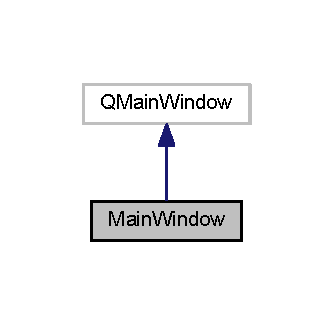
\includegraphics[width=160pt]{class_main_window__inherit__graph}
\end{center}
\end{figure}


Collaboration diagram for Main\+Window\+:\nopagebreak
\begin{figure}[H]
\begin{center}
\leavevmode
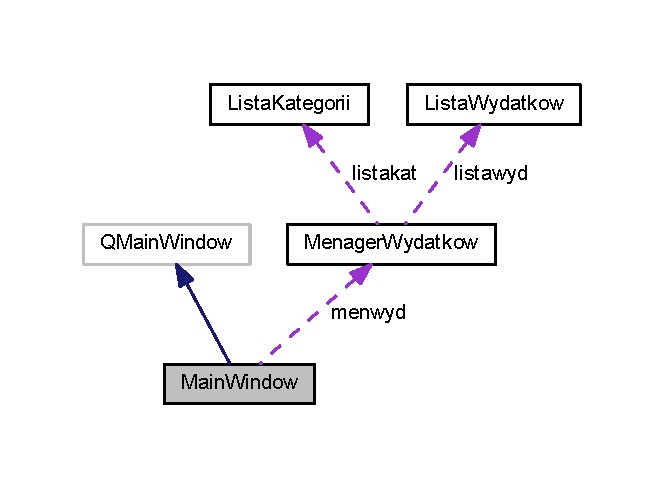
\includegraphics[width=319pt]{class_main_window__coll__graph}
\end{center}
\end{figure}
\subsection*{Public Member Functions}
\begin{DoxyCompactItemize}
\item 
\hyperlink{class_main_window_a8b244be8b7b7db1b08de2a2acb9409db}{Main\+Window} (Q\+Widget $\ast$parent=0)
\begin{DoxyCompactList}\small\item\em Konstruktor \hyperlink{class_main_window}{Main\+Window}. \end{DoxyCompactList}\end{DoxyCompactItemize}
\subsection*{Public Attributes}
\begin{DoxyCompactItemize}
\item 
\hypertarget{class_main_window_a342ff38f23b83c7da4f0cffa5b85c8ea}{}\hyperlink{class_menager_wydatkow}{Menager\+Wydatkow} \hyperlink{class_main_window_a342ff38f23b83c7da4f0cffa5b85c8ea}{menwyd}\label{class_main_window_a342ff38f23b83c7da4f0cffa5b85c8ea}

\begin{DoxyCompactList}\small\item\em Obiekt menwyd typu \hyperlink{class_menager_wydatkow}{Menager\+Wydatkow}. \end{DoxyCompactList}\end{DoxyCompactItemize}


\subsection{Detailed Description}
Klasa \hyperlink{class_main_window}{Main\+Window}. Klasa wyswietlajaca okno glowne. 

\subsection{Constructor \& Destructor Documentation}
\hypertarget{class_main_window_a8b244be8b7b7db1b08de2a2acb9409db}{}\index{Main\+Window@{Main\+Window}!Main\+Window@{Main\+Window}}
\index{Main\+Window@{Main\+Window}!Main\+Window@{Main\+Window}}
\subsubsection[{Main\+Window}]{\setlength{\rightskip}{0pt plus 5cm}Main\+Window\+::\+Main\+Window (
\begin{DoxyParamCaption}
\item[{Q\+Widget $\ast$}]{parent = {\ttfamily 0}}
\end{DoxyParamCaption}
)\hspace{0.3cm}{\ttfamily [explicit]}}\label{class_main_window_a8b244be8b7b7db1b08de2a2acb9409db}


Konstruktor \hyperlink{class_main_window}{Main\+Window}. 


\begin{DoxyParams}{Parameters}
{\em parent} & \\
\hline
\end{DoxyParams}


The documentation for this class was generated from the following files\+:\begin{DoxyCompactItemize}
\item 
mainwindow.\+h\item 
mainwindow.\+cpp\end{DoxyCompactItemize}

\hypertarget{class_menager_wydatkow}{}\section{Menager\+Wydatkow Class Reference}
\label{class_menager_wydatkow}\index{Menager\+Wydatkow@{Menager\+Wydatkow}}


Klasa \hyperlink{class_menager_wydatkow}{Menager\+Wydatkow}. Klasa zawierajaca wszystkie listy i laczaca sie z baza.  




{\ttfamily \#include $<$menagerwydatkow.\+h$>$}



Collaboration diagram for Menager\+Wydatkow\+:\nopagebreak
\begin{figure}[H]
\begin{center}
\leavevmode
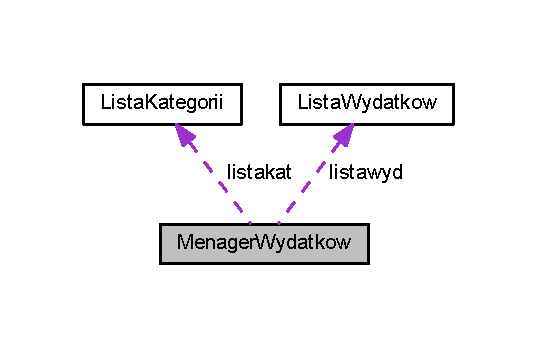
\includegraphics[width=258pt]{class_menager_wydatkow__coll__graph}
\end{center}
\end{figure}
\subsection*{Public Member Functions}
\begin{DoxyCompactItemize}
\item 
\hypertarget{class_menager_wydatkow_abf10a3d0748daf04ee787e67a642b09a}{}\hyperlink{class_menager_wydatkow_abf10a3d0748daf04ee787e67a642b09a}{Menager\+Wydatkow} ()\label{class_menager_wydatkow_abf10a3d0748daf04ee787e67a642b09a}

\begin{DoxyCompactList}\small\item\em Konstruktor \hyperlink{class_menager_wydatkow}{Menager\+Wydatkow}. \end{DoxyCompactList}\item 
bool \hyperlink{class_menager_wydatkow_af51b71d9b3da677b9b441f778f230a5f}{polacz\+D\+B} ()
\begin{DoxyCompactList}\small\item\em Funkcja polacz\+D\+B. Laczy sie z baza. \end{DoxyCompactList}\item 
\hypertarget{class_menager_wydatkow_a966523a5f411ad1f863ab0e0ca86b97e}{}void \hyperlink{class_menager_wydatkow_a966523a5f411ad1f863ab0e0ca86b97e}{wczytaj\+Liste\+Wydatkow\+D\+B} ()\label{class_menager_wydatkow_a966523a5f411ad1f863ab0e0ca86b97e}

\begin{DoxyCompactList}\small\item\em Funkcja wczytaj\+Liste\+Wydatkow\+D\+B. Wczytuje liste wydatkow z bazy. \end{DoxyCompactList}\item 
void \hyperlink{class_menager_wydatkow_aeaf79dc220332741e81cc073b08d6610}{wczytaj\+Liste\+Zestawienia\+D\+B} (Q\+Date start, Q\+Date koniec)
\begin{DoxyCompactList}\small\item\em Funkcja wczytaj\+Liste\+Zestawienia\+D\+B. Wczytuje liste zestawienia wydatkow z bazy, dla podanego okresu czasu. \end{DoxyCompactList}\item 
void \hyperlink{class_menager_wydatkow_a344d520de55e5134b589ba02300b9431}{wczytaj\+Sume\+Za\+Okres\+D\+B} (Q\+Date start, Q\+Date koniec)
\begin{DoxyCompactList}\small\item\em Funkcja wczytaj\+Sume\+Za\+Okres\+D\+B. Podaje sume wydatkow za okres. \end{DoxyCompactList}\item 
\hypertarget{class_menager_wydatkow_ae9a6ed4e74e93d8873129e8a8de2899f}{}void \hyperlink{class_menager_wydatkow_ae9a6ed4e74e93d8873129e8a8de2899f}{wczytaj\+Sume\+Calosci\+D\+B} ()\label{class_menager_wydatkow_ae9a6ed4e74e93d8873129e8a8de2899f}

\begin{DoxyCompactList}\small\item\em Funkcja wczytaj\+Sume\+Calosci\+D\+B. Podaje sume wydatkow za caly okres. \end{DoxyCompactList}\item 
void \hyperlink{class_menager_wydatkow_a30be73243e008dc5f7ab8eb669a05e55}{dodaj\+Wydatek} (Q\+String \+\_\+kategoria, Q\+Date \+\_\+data, double \+\_\+kwota, Q\+String \+\_\+opis)
\begin{DoxyCompactList}\small\item\em Funkcja dodaj\+Wydatek. Funkcja dodajaca wpis. \end{DoxyCompactList}\item 
void \hyperlink{class_menager_wydatkow_addeab8e73a7c13b9e4349892d692dfc3}{edytuj\+Wydatek} (int id, Q\+String kategoria, Q\+Date data, double kwota, Q\+String opis)
\begin{DoxyCompactList}\small\item\em Funkcja edytuj\+Wydatek. Umozliwia edycje wpisu. \end{DoxyCompactList}\item 
void \hyperlink{class_menager_wydatkow_a9aabc079d73f31d46a96148f85b9c4d7}{usun\+Wydatek} (int id)
\begin{DoxyCompactList}\small\item\em Funkcja usun\+Wydatek. Umozliwia usuwanie wpisu. \end{DoxyCompactList}\end{DoxyCompactItemize}
\subsection*{Public Attributes}
\begin{DoxyCompactItemize}
\item 
\hypertarget{class_menager_wydatkow_a3c981ccfc77f7f37e0d64c2a3897a7d0}{}\hyperlink{class_lista_wydatkow}{Lista\+Wydatkow} \hyperlink{class_menager_wydatkow_a3c981ccfc77f7f37e0d64c2a3897a7d0}{listawyd}\label{class_menager_wydatkow_a3c981ccfc77f7f37e0d64c2a3897a7d0}

\begin{DoxyCompactList}\small\item\em Obiekt listawyd typu \hyperlink{class_lista_wydatkow}{Lista\+Wydatkow}. \end{DoxyCompactList}\item 
\hypertarget{class_menager_wydatkow_a743a1a6ee65317e05e0efda038f2e104}{}\hyperlink{class_lista_kategorii}{Lista\+Kategorii} \hyperlink{class_menager_wydatkow_a743a1a6ee65317e05e0efda038f2e104}{listakat}\label{class_menager_wydatkow_a743a1a6ee65317e05e0efda038f2e104}

\begin{DoxyCompactList}\small\item\em Obiekt listakat typu \hyperlink{class_lista_kategorii}{Lista\+Kategorii}. \end{DoxyCompactList}\item 
\hypertarget{class_menager_wydatkow_a86bfd62a21e66b68a7f94550398a13a1}{}Q\+List$<$ \hyperlink{class_wpis_zestawienia}{Wpis\+Zestawienia} $>$ \hyperlink{class_menager_wydatkow_a86bfd62a21e66b68a7f94550398a13a1}{lista\+Zestawienia}\label{class_menager_wydatkow_a86bfd62a21e66b68a7f94550398a13a1}

\begin{DoxyCompactList}\small\item\em Obiekt lista\+Zestawienia typu Q\+List. \end{DoxyCompactList}\item 
\hypertarget{class_menager_wydatkow_a7f7d9dbb9e0ab215b725eff718596e10}{}double \hyperlink{class_menager_wydatkow_a7f7d9dbb9e0ab215b725eff718596e10}{suma\+Za\+Okres}\label{class_menager_wydatkow_a7f7d9dbb9e0ab215b725eff718596e10}

\begin{DoxyCompactList}\small\item\em Zmienna suma\+Za\+Okres typu double. \end{DoxyCompactList}\item 
\hypertarget{class_menager_wydatkow_a5620729078154b1911a15c999ddb87e9}{}double \hyperlink{class_menager_wydatkow_a5620729078154b1911a15c999ddb87e9}{suma\+Calosci}\label{class_menager_wydatkow_a5620729078154b1911a15c999ddb87e9}

\begin{DoxyCompactList}\small\item\em Zmienna suma\+Calosci typu double. \end{DoxyCompactList}\end{DoxyCompactItemize}


\subsection{Detailed Description}
Klasa \hyperlink{class_menager_wydatkow}{Menager\+Wydatkow}. Klasa zawierajaca wszystkie listy i laczaca sie z baza. 

\subsection{Member Function Documentation}
\hypertarget{class_menager_wydatkow_a30be73243e008dc5f7ab8eb669a05e55}{}\index{Menager\+Wydatkow@{Menager\+Wydatkow}!dodaj\+Wydatek@{dodaj\+Wydatek}}
\index{dodaj\+Wydatek@{dodaj\+Wydatek}!Menager\+Wydatkow@{Menager\+Wydatkow}}
\subsubsection[{dodaj\+Wydatek}]{\setlength{\rightskip}{0pt plus 5cm}void Menager\+Wydatkow\+::dodaj\+Wydatek (
\begin{DoxyParamCaption}
\item[{Q\+String}]{\+\_\+kategoria, }
\item[{Q\+Date}]{\+\_\+data, }
\item[{double}]{\+\_\+kwota, }
\item[{Q\+String}]{\+\_\+opis}
\end{DoxyParamCaption}
)}\label{class_menager_wydatkow_a30be73243e008dc5f7ab8eb669a05e55}


Funkcja dodaj\+Wydatek. Funkcja dodajaca wpis. 


\begin{DoxyParams}{Parameters}
{\em Argument} & \+\_\+kategoria typu Q\+String. \\
\hline
{\em Argument} & \+\_\+data typu Q\+Date. \\
\hline
{\em Argument} & \+\_\+kwota typu double. \\
\hline
{\em Argument} & \+\_\+opis typu Q\+String. \\
\hline
\end{DoxyParams}
\hypertarget{class_menager_wydatkow_addeab8e73a7c13b9e4349892d692dfc3}{}\index{Menager\+Wydatkow@{Menager\+Wydatkow}!edytuj\+Wydatek@{edytuj\+Wydatek}}
\index{edytuj\+Wydatek@{edytuj\+Wydatek}!Menager\+Wydatkow@{Menager\+Wydatkow}}
\subsubsection[{edytuj\+Wydatek}]{\setlength{\rightskip}{0pt plus 5cm}void Menager\+Wydatkow\+::edytuj\+Wydatek (
\begin{DoxyParamCaption}
\item[{int}]{id, }
\item[{Q\+String}]{kategoria, }
\item[{Q\+Date}]{data, }
\item[{double}]{kwota, }
\item[{Q\+String}]{opis}
\end{DoxyParamCaption}
)}\label{class_menager_wydatkow_addeab8e73a7c13b9e4349892d692dfc3}


Funkcja edytuj\+Wydatek. Umozliwia edycje wpisu. 


\begin{DoxyParams}{Parameters}
{\em Argument} & id typu int. \\
\hline
{\em Argument} & kategoria typu Q\+String. \\
\hline
{\em Argument} & data typu Q\+Date. \\
\hline
{\em Argument} & kwota typu double. \\
\hline
{\em Argument} & opis typu Q\+String. \\
\hline
\end{DoxyParams}
\hypertarget{class_menager_wydatkow_af51b71d9b3da677b9b441f778f230a5f}{}\index{Menager\+Wydatkow@{Menager\+Wydatkow}!polacz\+D\+B@{polacz\+D\+B}}
\index{polacz\+D\+B@{polacz\+D\+B}!Menager\+Wydatkow@{Menager\+Wydatkow}}
\subsubsection[{polacz\+D\+B}]{\setlength{\rightskip}{0pt plus 5cm}bool Menager\+Wydatkow\+::polacz\+D\+B (
\begin{DoxyParamCaption}
{}
\end{DoxyParamCaption}
)}\label{class_menager_wydatkow_af51b71d9b3da677b9b441f778f230a5f}


Funkcja polacz\+D\+B. Laczy sie z baza. 

\begin{DoxyReturn}{Returns}
Zwraca zmienna typu bool. 
\end{DoxyReturn}
\hypertarget{class_menager_wydatkow_a9aabc079d73f31d46a96148f85b9c4d7}{}\index{Menager\+Wydatkow@{Menager\+Wydatkow}!usun\+Wydatek@{usun\+Wydatek}}
\index{usun\+Wydatek@{usun\+Wydatek}!Menager\+Wydatkow@{Menager\+Wydatkow}}
\subsubsection[{usun\+Wydatek}]{\setlength{\rightskip}{0pt plus 5cm}void Menager\+Wydatkow\+::usun\+Wydatek (
\begin{DoxyParamCaption}
\item[{int}]{id}
\end{DoxyParamCaption}
)}\label{class_menager_wydatkow_a9aabc079d73f31d46a96148f85b9c4d7}


Funkcja usun\+Wydatek. Umozliwia usuwanie wpisu. 


\begin{DoxyParams}{Parameters}
{\em Argument} & id typu int. \\
\hline
\end{DoxyParams}
\hypertarget{class_menager_wydatkow_aeaf79dc220332741e81cc073b08d6610}{}\index{Menager\+Wydatkow@{Menager\+Wydatkow}!wczytaj\+Liste\+Zestawienia\+D\+B@{wczytaj\+Liste\+Zestawienia\+D\+B}}
\index{wczytaj\+Liste\+Zestawienia\+D\+B@{wczytaj\+Liste\+Zestawienia\+D\+B}!Menager\+Wydatkow@{Menager\+Wydatkow}}
\subsubsection[{wczytaj\+Liste\+Zestawienia\+D\+B}]{\setlength{\rightskip}{0pt plus 5cm}void Menager\+Wydatkow\+::wczytaj\+Liste\+Zestawienia\+D\+B (
\begin{DoxyParamCaption}
\item[{Q\+Date}]{start, }
\item[{Q\+Date}]{koniec}
\end{DoxyParamCaption}
)}\label{class_menager_wydatkow_aeaf79dc220332741e81cc073b08d6610}


Funkcja wczytaj\+Liste\+Zestawienia\+D\+B. Wczytuje liste zestawienia wydatkow z bazy, dla podanego okresu czasu. 


\begin{DoxyParams}{Parameters}
{\em Argument} & start typu Q\+Date. \\
\hline
{\em Argument} & koniec typu Q\+Date. \\
\hline
\end{DoxyParams}
\hypertarget{class_menager_wydatkow_a344d520de55e5134b589ba02300b9431}{}\index{Menager\+Wydatkow@{Menager\+Wydatkow}!wczytaj\+Sume\+Za\+Okres\+D\+B@{wczytaj\+Sume\+Za\+Okres\+D\+B}}
\index{wczytaj\+Sume\+Za\+Okres\+D\+B@{wczytaj\+Sume\+Za\+Okres\+D\+B}!Menager\+Wydatkow@{Menager\+Wydatkow}}
\subsubsection[{wczytaj\+Sume\+Za\+Okres\+D\+B}]{\setlength{\rightskip}{0pt plus 5cm}void Menager\+Wydatkow\+::wczytaj\+Sume\+Za\+Okres\+D\+B (
\begin{DoxyParamCaption}
\item[{Q\+Date}]{start, }
\item[{Q\+Date}]{koniec}
\end{DoxyParamCaption}
)}\label{class_menager_wydatkow_a344d520de55e5134b589ba02300b9431}


Funkcja wczytaj\+Sume\+Za\+Okres\+D\+B. Podaje sume wydatkow za okres. 


\begin{DoxyParams}{Parameters}
{\em Argument} & start typu Q\+Date. \\
\hline
{\em Argument} & koniec typu Q\+Date. \\
\hline
\end{DoxyParams}


The documentation for this class was generated from the following files\+:\begin{DoxyCompactItemize}
\item 
menagerwydatkow.\+h\item 
menagerwydatkow.\+cpp\end{DoxyCompactItemize}

\hypertarget{class_wpis_zestawienia}{}\section{Wpis\+Zestawienia Class Reference}
\label{class_wpis_zestawienia}\index{Wpis\+Zestawienia@{Wpis\+Zestawienia}}


Klasa \hyperlink{class_wpis_zestawienia}{Wpis\+Zestawienia}. Klasa reprezentujaca pojedynczy wpis z zestawienia.  




{\ttfamily \#include $<$wpiszestawienia.\+h$>$}

\subsection*{Public Member Functions}
\begin{DoxyCompactItemize}
\item 
\hypertarget{class_wpis_zestawienia_a2c7a512d73c0b2ea7aefea06e273b546}{}\hyperlink{class_wpis_zestawienia_a2c7a512d73c0b2ea7aefea06e273b546}{Wpis\+Zestawienia} ()\label{class_wpis_zestawienia_a2c7a512d73c0b2ea7aefea06e273b546}

\begin{DoxyCompactList}\small\item\em Konstruktor \hyperlink{class_wpis_zestawienia}{Wpis\+Zestawienia}. \end{DoxyCompactList}\item 
\hyperlink{class_wpis_zestawienia_aff55225999605924177b3c2f5000ff86}{Wpis\+Zestawienia} (Q\+Date \hyperlink{class_wpis_zestawienia_a5d457906aef5d46dc6ee4744a1851cb3}{start}, Q\+Date \hyperlink{class_wpis_zestawienia_a3575567bd1069656acc3a39b193d7500}{koniec}, Q\+String \hyperlink{class_wpis_zestawienia_a286d6a98e6b41c38e6891bf71a474f47}{kategoria}, int \hyperlink{class_wpis_zestawienia_af8437e93134f18328e37e2fe05b3c7f5}{ilosc}, double \hyperlink{class_wpis_zestawienia_a3128b0bac6d69ea0db7ccc200adc6188}{suma})
\begin{DoxyCompactList}\small\item\em Konstruktor \hyperlink{class_wpis_zestawienia}{Wpis\+Zestawienia}. \end{DoxyCompactList}\item 
\hypertarget{class_wpis_zestawienia_a39c99052b33bffbd6dc07e425dd19a76}{}void \hyperlink{class_wpis_zestawienia_a39c99052b33bffbd6dc07e425dd19a76}{print} ()\label{class_wpis_zestawienia_a39c99052b33bffbd6dc07e425dd19a76}

\begin{DoxyCompactList}\small\item\em Funkcja print. Wyswietla wpis zestawienia. \end{DoxyCompactList}\end{DoxyCompactItemize}
\subsection*{Public Attributes}
\begin{DoxyCompactItemize}
\item 
\hypertarget{class_wpis_zestawienia_a5d457906aef5d46dc6ee4744a1851cb3}{}Q\+Date \hyperlink{class_wpis_zestawienia_a5d457906aef5d46dc6ee4744a1851cb3}{start}\label{class_wpis_zestawienia_a5d457906aef5d46dc6ee4744a1851cb3}

\begin{DoxyCompactList}\small\item\em Obiekt start typu Q\+Date. \end{DoxyCompactList}\item 
\hypertarget{class_wpis_zestawienia_a3575567bd1069656acc3a39b193d7500}{}Q\+Date \hyperlink{class_wpis_zestawienia_a3575567bd1069656acc3a39b193d7500}{koniec}\label{class_wpis_zestawienia_a3575567bd1069656acc3a39b193d7500}

\begin{DoxyCompactList}\small\item\em Obiekt koniec typu Q\+Date. \end{DoxyCompactList}\item 
\hypertarget{class_wpis_zestawienia_a286d6a98e6b41c38e6891bf71a474f47}{}Q\+String \hyperlink{class_wpis_zestawienia_a286d6a98e6b41c38e6891bf71a474f47}{kategoria}\label{class_wpis_zestawienia_a286d6a98e6b41c38e6891bf71a474f47}

\begin{DoxyCompactList}\small\item\em Obiekt kategoria typu Q\+String. \end{DoxyCompactList}\item 
\hypertarget{class_wpis_zestawienia_af8437e93134f18328e37e2fe05b3c7f5}{}int \hyperlink{class_wpis_zestawienia_af8437e93134f18328e37e2fe05b3c7f5}{ilosc}\label{class_wpis_zestawienia_af8437e93134f18328e37e2fe05b3c7f5}

\begin{DoxyCompactList}\small\item\em Zmienna ilosc typu int. \end{DoxyCompactList}\item 
\hypertarget{class_wpis_zestawienia_a3128b0bac6d69ea0db7ccc200adc6188}{}double \hyperlink{class_wpis_zestawienia_a3128b0bac6d69ea0db7ccc200adc6188}{suma}\label{class_wpis_zestawienia_a3128b0bac6d69ea0db7ccc200adc6188}

\begin{DoxyCompactList}\small\item\em Zmienna suma typu double. \end{DoxyCompactList}\end{DoxyCompactItemize}


\subsection{Detailed Description}
Klasa \hyperlink{class_wpis_zestawienia}{Wpis\+Zestawienia}. Klasa reprezentujaca pojedynczy wpis z zestawienia. 

\subsection{Constructor \& Destructor Documentation}
\hypertarget{class_wpis_zestawienia_aff55225999605924177b3c2f5000ff86}{}\index{Wpis\+Zestawienia@{Wpis\+Zestawienia}!Wpis\+Zestawienia@{Wpis\+Zestawienia}}
\index{Wpis\+Zestawienia@{Wpis\+Zestawienia}!Wpis\+Zestawienia@{Wpis\+Zestawienia}}
\subsubsection[{Wpis\+Zestawienia}]{\setlength{\rightskip}{0pt plus 5cm}Wpis\+Zestawienia\+::\+Wpis\+Zestawienia (
\begin{DoxyParamCaption}
\item[{Q\+Date}]{start, }
\item[{Q\+Date}]{koniec, }
\item[{Q\+String}]{kategoria, }
\item[{int}]{ilosc, }
\item[{double}]{suma}
\end{DoxyParamCaption}
)}\label{class_wpis_zestawienia_aff55225999605924177b3c2f5000ff86}


Konstruktor \hyperlink{class_wpis_zestawienia}{Wpis\+Zestawienia}. 


\begin{DoxyParams}{Parameters}
{\em Argument} & start typu Q\+Date. \\
\hline
{\em Argument} & koniec typu Q\+Date. \\
\hline
{\em Argument} & kategoria typu Q\+String. \\
\hline
{\em Argument} & ilosc typu int. \\
\hline
{\em Argument} & suma typu double. \\
\hline
\end{DoxyParams}


The documentation for this class was generated from the following files\+:\begin{DoxyCompactItemize}
\item 
wpiszestawienia.\+h\item 
wpiszestawienia.\+cpp\end{DoxyCompactItemize}

\hypertarget{class_wydatek}{}\section{Wydatek Class Reference}
\label{class_wydatek}\index{Wydatek@{Wydatek}}


Klasa \hyperlink{class_wydatek}{Wydatek}. Klasa reprezentujaca pojedynczy wpis.  




{\ttfamily \#include $<$wydatek.\+h$>$}

\subsection*{Public Member Functions}
\begin{DoxyCompactItemize}
\item 
\hypertarget{class_wydatek_a7588555254ce5ac1b84a3a7a52114a92}{}\hyperlink{class_wydatek_a7588555254ce5ac1b84a3a7a52114a92}{Wydatek} ()\label{class_wydatek_a7588555254ce5ac1b84a3a7a52114a92}

\begin{DoxyCompactList}\small\item\em K\+Onstruktor \hyperlink{class_wydatek}{Wydatek}. \end{DoxyCompactList}\item 
\hyperlink{class_wydatek_aaadfcce4a0c183388bfb9a2e8a1e5f4a}{Wydatek} (unsigned int \hyperlink{class_wydatek_aaa67349adee2d242127ca4e7114e800b}{I\+D}, Q\+Date \hyperlink{class_wydatek_a711d55393993069d2795f0d545de64d1}{data}, Q\+String \hyperlink{class_wydatek_a39c836807249ffa4c683455b5ef8b2a0}{kategoria}, double \hyperlink{class_wydatek_a1786e869ea300a3a9d2cef7e89a10419}{kwota}, Q\+String \hyperlink{class_wydatek_ac9ea73c7ca92621388756045fb467881}{opis})
\begin{DoxyCompactList}\small\item\em Konstruktor \hyperlink{class_wydatek}{Wydatek}. \end{DoxyCompactList}\item 
\hypertarget{class_wydatek_a175492204adf6f5c4f2da52ea095fe60}{}void \hyperlink{class_wydatek_a175492204adf6f5c4f2da52ea095fe60}{print} ()\label{class_wydatek_a175492204adf6f5c4f2da52ea095fe60}

\begin{DoxyCompactList}\small\item\em Funkcja print. Wyswietla wpis. \end{DoxyCompactList}\end{DoxyCompactItemize}
\subsection*{Public Attributes}
\begin{DoxyCompactItemize}
\item 
\hypertarget{class_wydatek_aaa67349adee2d242127ca4e7114e800b}{}unsigned int \hyperlink{class_wydatek_aaa67349adee2d242127ca4e7114e800b}{I\+D}\label{class_wydatek_aaa67349adee2d242127ca4e7114e800b}

\begin{DoxyCompactList}\small\item\em Zmienna I\+D typu unsigned int. \end{DoxyCompactList}\item 
\hypertarget{class_wydatek_a711d55393993069d2795f0d545de64d1}{}Q\+Date \hyperlink{class_wydatek_a711d55393993069d2795f0d545de64d1}{data}\label{class_wydatek_a711d55393993069d2795f0d545de64d1}

\begin{DoxyCompactList}\small\item\em Obiekt data typu Q\+Date. \end{DoxyCompactList}\item 
\hypertarget{class_wydatek_a39c836807249ffa4c683455b5ef8b2a0}{}Q\+String \hyperlink{class_wydatek_a39c836807249ffa4c683455b5ef8b2a0}{kategoria}\label{class_wydatek_a39c836807249ffa4c683455b5ef8b2a0}

\begin{DoxyCompactList}\small\item\em Obiekt kategoria typu Q\+String. \end{DoxyCompactList}\item 
\hypertarget{class_wydatek_a1786e869ea300a3a9d2cef7e89a10419}{}double \hyperlink{class_wydatek_a1786e869ea300a3a9d2cef7e89a10419}{kwota}\label{class_wydatek_a1786e869ea300a3a9d2cef7e89a10419}

\begin{DoxyCompactList}\small\item\em Zmienna kwota typu double. \end{DoxyCompactList}\item 
\hypertarget{class_wydatek_ac9ea73c7ca92621388756045fb467881}{}Q\+String \hyperlink{class_wydatek_ac9ea73c7ca92621388756045fb467881}{opis}\label{class_wydatek_ac9ea73c7ca92621388756045fb467881}

\begin{DoxyCompactList}\small\item\em Obiekt opis typu Q\+String. \end{DoxyCompactList}\end{DoxyCompactItemize}


\subsection{Detailed Description}
Klasa \hyperlink{class_wydatek}{Wydatek}. Klasa reprezentujaca pojedynczy wpis. 

\subsection{Constructor \& Destructor Documentation}
\hypertarget{class_wydatek_aaadfcce4a0c183388bfb9a2e8a1e5f4a}{}\index{Wydatek@{Wydatek}!Wydatek@{Wydatek}}
\index{Wydatek@{Wydatek}!Wydatek@{Wydatek}}
\subsubsection[{Wydatek}]{\setlength{\rightskip}{0pt plus 5cm}Wydatek\+::\+Wydatek (
\begin{DoxyParamCaption}
\item[{unsigned int}]{I\+D, }
\item[{Q\+Date}]{data, }
\item[{Q\+String}]{kategoria, }
\item[{double}]{kwota, }
\item[{Q\+String}]{opis}
\end{DoxyParamCaption}
)}\label{class_wydatek_aaadfcce4a0c183388bfb9a2e8a1e5f4a}


Konstruktor \hyperlink{class_wydatek}{Wydatek}. 


\begin{DoxyParams}{Parameters}
{\em Argument} & I\+D typu int. \\
\hline
{\em Argument} & data typu Q\+Date. \\
\hline
{\em Argument} & kategoria typu Q\+String. \\
\hline
{\em Argument} & kwota typu double. \\
\hline
{\em Argument} & opis typu Q\+String. \\
\hline
\end{DoxyParams}


The documentation for this class was generated from the following files\+:\begin{DoxyCompactItemize}
\item 
wydatek.\+h\item 
wydatek.\+cpp\end{DoxyCompactItemize}

\hypertarget{class_zestawienie}{}\section{Zestawienie Class Reference}
\label{class_zestawienie}\index{Zestawienie@{Zestawienie}}


The documentation for this class was generated from the following files\+:\begin{DoxyCompactItemize}
\item 
zestawienie.\+h\item 
zestawienie.\+cpp\end{DoxyCompactItemize}

%--- End generated contents ---

% Index
\backmatter
\newpage
\phantomsection
\clearemptydoublepage
\addcontentsline{toc}{chapter}{Index}
\printindex

\end{document}
